\chapter{METODE PENELITIAN}
\section{Tempat dan Waktu Penelitian}
Penelitian ini dilaksanakan dari bulan Februari 2025 hingga Juni
2025, bertempat di Laboratorium Elektronika dan Instrumentasi,
Departemen Fisika, Fakultas Matematika dan Ilmu Pengetahuan Alam,
Universitas Hasanuddin, Makassar.

\vspace{1em}

\section{Peralatan Penelitian}
Peralatan yang digunakan pada penelitian ini adalah sebagai berikut:
\begin{enumerate}
  \item Arduino Uno. berfungsi sebagai mikrokontroler utama yang
    mengendalikan motor \textit{servo} pada lengan robot dan menerima
    sinyal dari sensor.
  \item Motor \textit{servo}, digunakan sebagai aktuator untuk
    menggerakkan bagian-bagian lengan robot sesuai perintah dari Arduino.
  \item Lengan robot EEZYbotARM MK1, merupakan struktur
    mekanik  tempat pemasangan motor \textit{servo} dan berperan
    sebagai sistem penggerak robotik.
  \item \textit{Power supply} 5V, berfungsi menyediakan tegangan
    stabil untuk pengoperasian motor \textit{servo} .
  \item \textit{Sensor Passive Infrared Receiver} (PIR) HC-SR501,
    digunakan untuk mendeteksi pergerakan dan membantu
    menghitung jumlah kontainer cacat dan maupun tidak cacat yang melintas.
  \item Kamera, digunakan untuk mengambil citra kontainer kimia, yang
    akan diproses oleh model deteksi objek (YOLO) dan deteksi kecacatan
    (\textit{autoencoder}).
  \item Laptop/komputer, digunakan untuk memuat program ke Arduino
    Uno, serta menjalankan model deteksi objek berbasis YOLO dan
    \textit{autoencoder} untuk analisis visual.
  \item Kabel \textit{jumper}, berfungsi menghubungkan berbagai komponen
    elektronik seperti sensor dan aktuator ke papan rangkaian dan
    Arduino.
  \item Papan rangkaian, berfungsi untuk menyediakan jalur koneksi
    antar komponen.
\end{enumerate}

\vspace{1em}

\section{Metode Kerja}
Penelitian ini terdiri dari beberapa tahapan, sebagaimana ditunjukkan
pada Gambar \ref{fig:bagan-umum}. Fokus penelitian ini adalah pada
perancangan dan pembuatan prototipe sistem deteksi cacat secara otomatis.

% \begin{figure}[H]
%   \centering
%   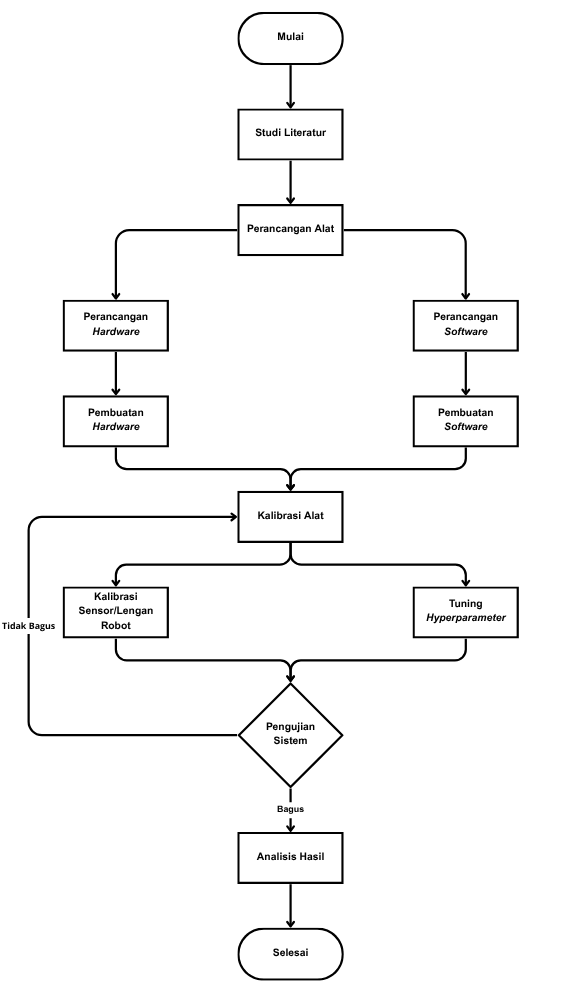
\includegraphics[width=0.7\textwidth]{gambar/bagan-umum.png}
%   \caption{Bagan alir penelitian}
%   \label{fig:bagan-umum}
% \end{figure}
% \vspace{-1em}

\begin{figure}[H]
  \centering
  \begin{tikzpicture}[
      every node/.style={font=\fontsize{9}{11}\selectfont},
      node distance = 0.77cm and 1cm
    ]
    \node (mulai) [startstop] {Mulai};
    \node (literatur) [process, below=of mulai] {Studi Literatur};
    \node (perancangan-alat) [process, below=of literatur] {Perancangan Alat};
    \node (perancangan-hardware) [process, align=center, below
    left=of perancangan-alat]
    {Perancangan \\ \textit{Hardware}};
    \node (perancangan-software) [process, align=center, below
    right=of perancangan-alat]
    {Perancangan \\ \textit{Software}};
    \node (pembuatan-hardware) [process, align=center, below=of
    perancangan-hardware]
    {Pembuatan \\ \textit{Hardware}};
    \node (pembuatan-software) [process, align=center, below=of
    perancangan-software]
    {Pembuatan \\ \textit{Software}};
    \coordinate (merge1) at
    ($(pembuatan-hardware.south)!0.5!(pembuatan-software.south)$);
    \node (kalibrasi-alat) [process, align=center, below=of merge1,
    yshift=-0.5cm] {Kalibrasi Alat};
    \node (kalibrasi-sensor) [process, align=center, below left=of
    kalibrasi-alat]
    {Kalibrasi \\ Sensor/Lengan Robot};
    \node (kalibrasi-parameter) [process, align=center, below
    right=of kalibrasi-alat]
    {\textit{Tuning} \\ \textit{Hyperparameter}};
    \coordinate (merge2) at
    ($(kalibrasi-sensor.south)!0.5!(kalibrasi-parameter.south)$);
    \node (pengujian-sistem) [decision, align=center, below=of
    merge2, yshift=-0.5cm] {Pengujian \\ Sistem};
    \node (analisis-hasil) [process, below=of pengujian-sistem]
    {Analisis Hasil};
    \node (selesai) [startstop, below=of analisis-hasil]
    {Selesai};

    % Arrow
    \draw [arrow] (mulai) -- (literatur);
    \draw [arrow] (literatur) -- (perancangan-alat);

    \draw [arrow] (perancangan-alat.west) -| (perancangan-hardware.north);
    \draw [arrow] (perancangan-alat.east) -| (perancangan-software.north);
    \draw [arrow] (perancangan-hardware) -- (pembuatan-hardware);
    \draw [arrow] (perancangan-software) -- (pembuatan-software);

    \draw [arrow] (pembuatan-hardware.south) --
    ($(pembuatan-hardware.south)+(0,-0.67cm)$) -| (kalibrasi-alat.north);
    \draw [arrow] (pembuatan-software.south) --
    ($(pembuatan-software.south)+(0,-0.67cm)$) -| (kalibrasi-alat.north);

    \draw [arrow] (kalibrasi-alat.south) --
    ($(kalibrasi-alat.south)+(0,-0.35cm)$) -| (kalibrasi-sensor.north);
    \draw [arrow] (kalibrasi-alat.south) --
    ($(kalibrasi-alat.south)+(0,-0.35cm)$) -| (kalibrasi-parameter.north);

    \draw [arrow] (kalibrasi-sensor.south) --
    ($(kalibrasi-sensor.south)+(0,-0.6cm)$) -| (pengujian-sistem.north);
    \draw [arrow] (kalibrasi-parameter.south) --
    ($(kalibrasi-parameter.south)+(0,-0.6cm)$) -| (pengujian-sistem.north);

    \draw [arrow] (pengujian-sistem.west) -- node[midway,
    yshift=0.25cm]{Tidak Bagus}
    ($(pengujian-sistem.west)+(-4.7cm,0)$) |- (kalibrasi-alat.west);
    \draw [arrow] (pengujian-sistem) -- node[midway, xshift=0.5cm]{Bagus}
    (analisis-hasil);

    \draw [arrow] (analisis-hasil) -- (selesai);

  \end{tikzpicture}
  \caption{Bagan alir penelitian}
  \label{fig:bagan-umum}
\end{figure}
\vspace{-1em}

Tahapan awal dimulai dengan kajian literatur mendalam mengenai
teknologi robotik, algoritma \textit{autoencoder} untuk deteksi anomali
visual, serta metode deteksi objek seperti YOLO. Kajian ini bertujuan
untuk memperoleh pemahaman komprehensif terkait format
\textit{dataset} dan perancangan model deteksi cacat pada kontainer
kimia. Setelah
pemahaman awal diperoleh, dilakukan perancangan sistem yang mencakup
komponen perangkat keras (lengan robot dan sensor) dan perangkat
lunak berupa algoritma \textit{machine learning}. Selanjutnya sistem
robot dikalibrasi agar dapat bekerja secara optimal, termasuk proses
\textit{tuning hyperparameter} pada model \textit{machine learning}
agar berfungsi secara
optimal. Setelah sistem dapat beroperasi dengan baik, dilakukan proses
pengambilan data sebagai langkah awal dalam pengujian dan validasi model.

\vspace{1em}

\subsection{Perancangan \textit{Hardware}}
Penelitian ini dimulai dengan tahap perancangan \textit{hardware}.
Komponen \textit{hardware} meliputi kamera untuk mengambil citra
kontainer kimia, laptop sebagai pusat pemrosesan algoritma, dan
sensor PIR untuk menghitung jumlah kontainer cacat dan tidak cacat.
Rangkaian \textit{hardware} dapat dilihat pada Gambar \ref{fig:rangkaian}.

\begin{figure}[H]
  \centering
  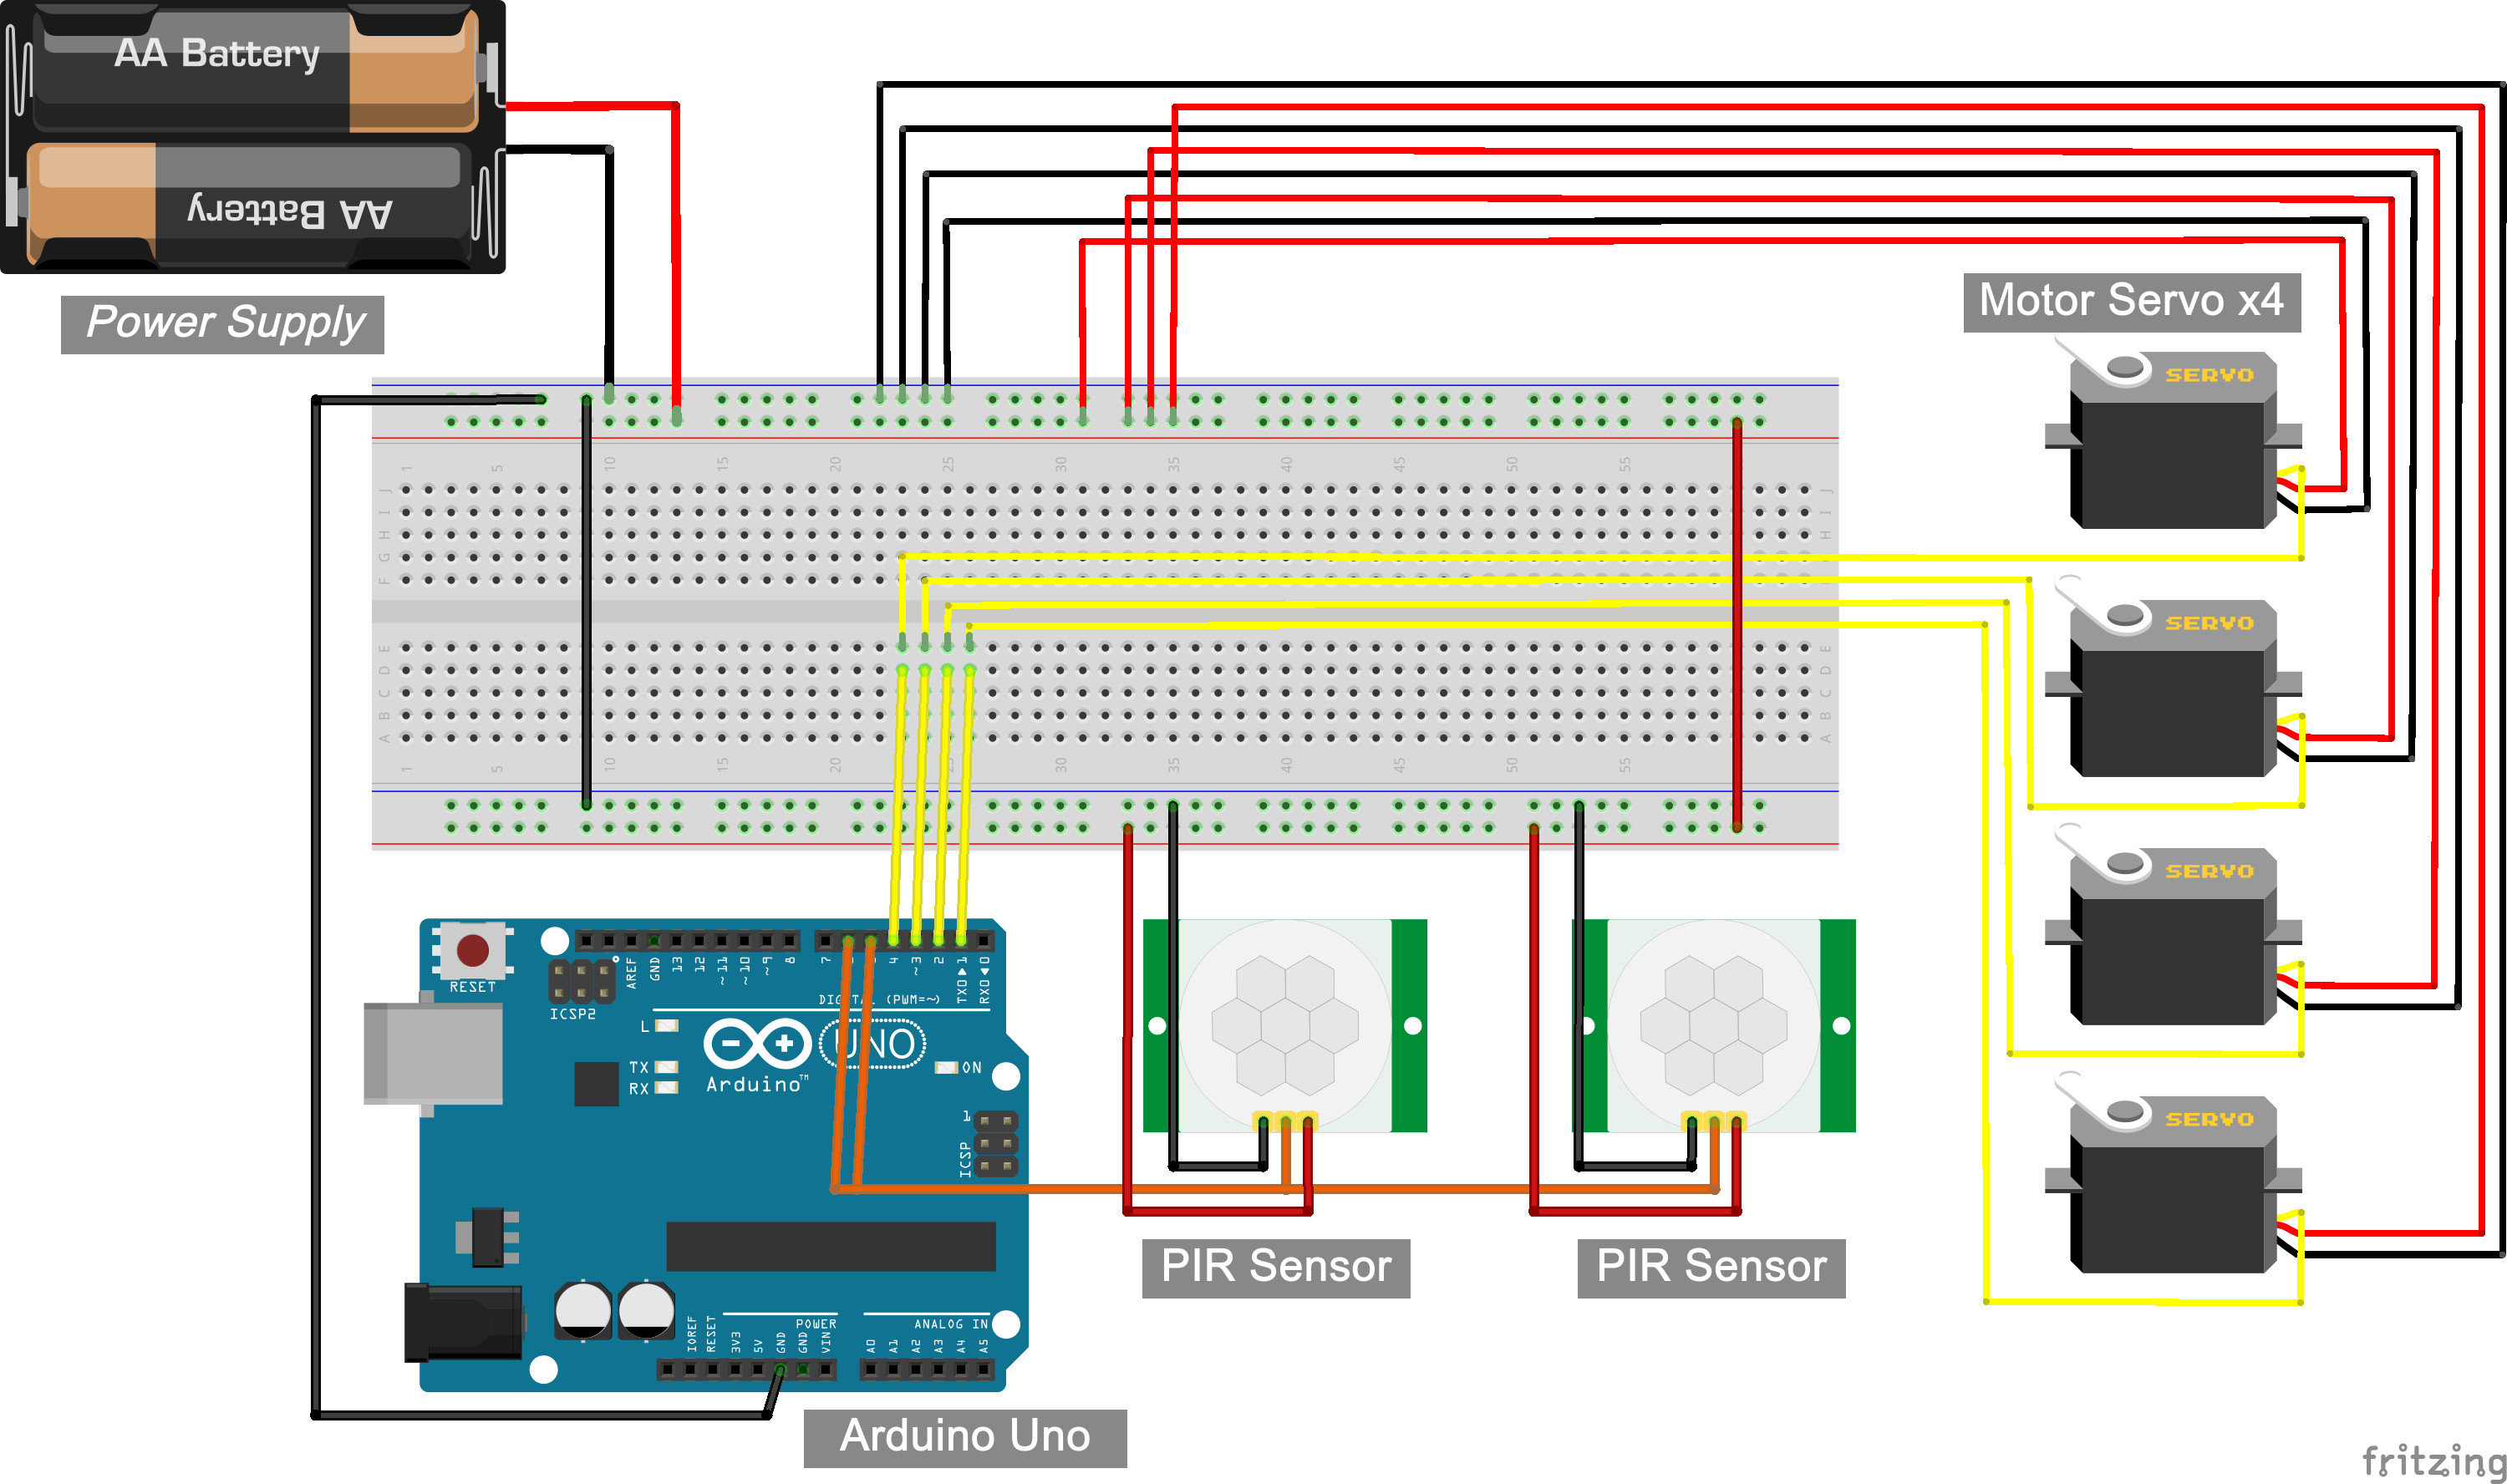
\includegraphics[width=\textwidth]{gambar/rangkaian.jpg}
  \caption{Rangkaian \textit{hardware} sistem}
  \label{fig:rangkaian}
\end{figure}
\vspace{-1em}

Alur kerja sistem dimulai saat kamera menangkap citra kontainer yang
berada pada area pengambilan gambar. Model YOLO digunakan untuk
mendeteksi objek kontainer. Setelah objek dikenali, citra dikirim ke
model deteksi kecacatan berbasis \textit{convolutional variational
autoencoder} (CVAE) untuk menentukan keberadaan cacat. Berdasarkan
hasil analisis tersebut, Arduino mengirimkan sinyal ke motor
\textit{servo} untuk menggerakkan lengan robot dalam memindahkan
kontainer sesuai
hasil klasifikasi. Dua sensor PIR yang dipasang pada masing-masing
wadah (cacat dan tidak cacat) digunakan untuk mencatat jumlah
kontainer. Data dari sensor dikirim \textit{server} dan ditampilkan
secara \textit{real-time}. Diagram  keterkaitan antar komponen
disajikan pada Gambar \ref{fig:hardware}.

\begin{figure}[H]
  \centering
  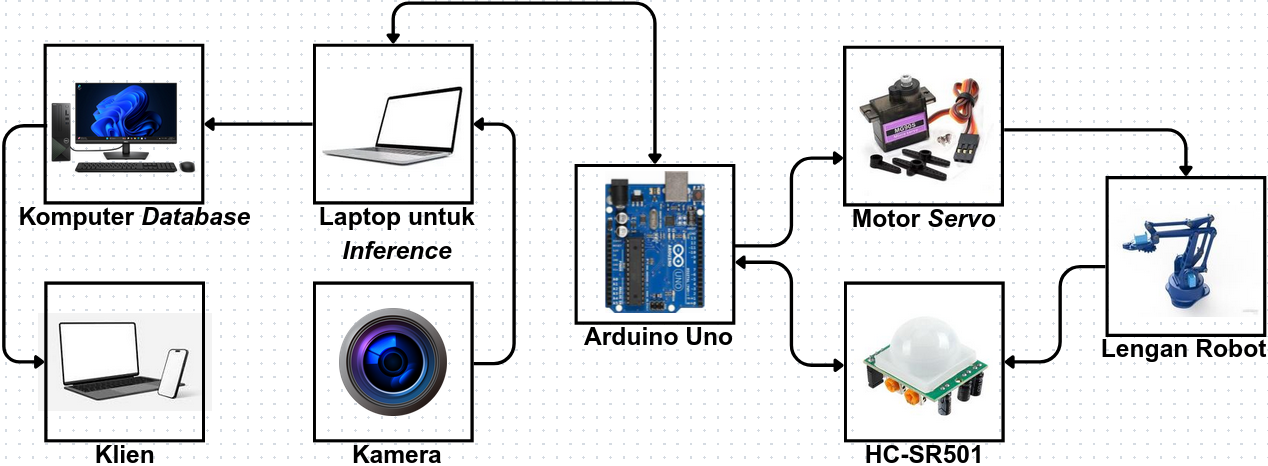
\includegraphics[width=\textwidth]{gambar/rancang.png}
  \caption{Rancang sistem \textit{hardware}}
  \label{fig:hardware}
\end{figure}
\vspace{-1em}

\vspace{1em}

\subsection{Perancangan \textit{Software}}
Perangkat lunak dalam penelitian ini mencakup: model deteksi objek
berbasis YOLO untuk mengidentifikasi kontainer kimia, kedua adalah
model deteksi cacat menggunakan CVAE, ketiga adalah algoritma kontrol
pergerakan lengan robot, dan yang keempat adalah integrasi modul
\textit{Internet of Things} (IoT) untuk menampilkan data secara
\textit{real-time} melalui \textit{website}.

Proses diawali dengan pengumpulan citra kontainer kimia dari berbagai
kondisi dan sudut pandang menggunakan kamera. \textit{Dataset} yang
diperoleh kemudian dianotasi secara manual dengan label dan
\textit{bounding box} format YOLO. Model dilatih untuk mendeteksi
kontainer secara akurat dan cepat. Evaluasi dilakukan menggunakan metrik
\textit{precision}, \textit{recall}, dan \textit{mean Average
Precision} (mAP), guna memastikan model memiliki kemampuan
generalisasi yang baik. Alur proses dapat dilihat pada Gambar
\ref{fig:pipeline-yolo}.

% \begin{figure}[H]
%   \centering
%   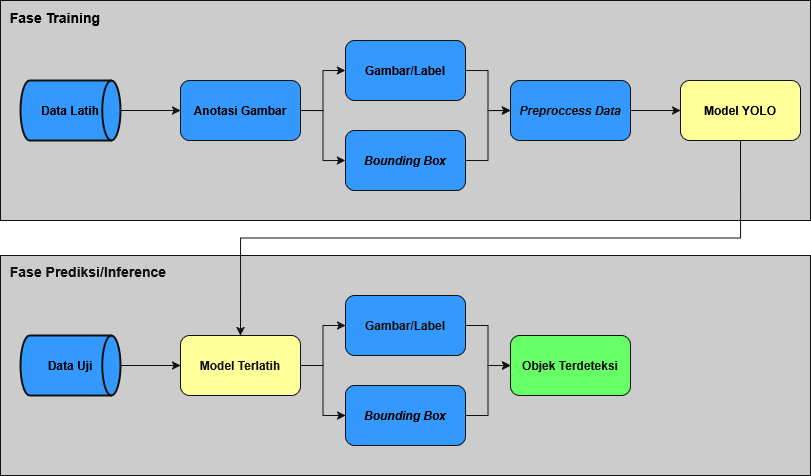
\includegraphics[width=\textwidth]{gambar/pipeline_yolo.png}
%   \caption{Diagram \textit{pipeline} pelatihan model YOLO}
%   \label{fig:pipeline-yolo}
% \end{figure}
% \vspace{-1em}

\begin{figure}[H]
  \centering
  \begin{tikzpicture}[
      every node/.style={font=\fontsize{8.5}{11}\selectfont},
      node distance = 0.5cm and 0.5cm
    ]
    % --- Pipeline pertama ---
    \node (data-latih1) [data] {Data Latih};
    \node (anotasi1) [pipeline-box, fill=cyan!50, right=of
    data-latih1] {Anotasi Gambar};
    \node (gambar-label1) [pipeline-box, fill=cyan!50, above right=of
    anotasi1] {Gambar/Label};
    \node (bounding-box1) [pipeline-box, fill=cyan!50, below right=of
    anotasi1] {\textit{Bounding Box}};
    \node (preprocess1) [pipeline-box, fill=cyan!50, above right=of
    bounding-box1] {\textit{Preprocess Data}};
    \node (yolo1) [pipeline-box, fill=yellow!50, right=of
    preprocess1] {Model Yolo};

    % Node dummy
    \node (start-bawah) [below=3cm of data-latih1] {};

    % --- Pipeline kedua ---
    \node (data-uji) [data, below=of start-bawah, xshift=1cm] {Data Uji};
    \node (model-terlatih) [pipeline-box, fill=yellow!50, right=of
    data-uji] {Model Terlatih};
    \node (gambar-label2) [pipeline-box, fill=cyan!50, above right=of
    model-terlatih] {Gambar/Label};
    \node (bounding-box2) [pipeline-box, fill=cyan!50, below right=of
    model-terlatih] {\textit{Bounding Box}};
    \node (objek-terdeteksi) [pipeline-box, fill=green!50, above
    right=of bounding-box2] {Objek Terdeteksi};

    % Arrow
    \draw [arrow] (data-latih1) -- (anotasi1);
    \draw [arrow] (anotasi1.east) -- ($(anotasi1.east)+(0.25cm, 0)$)
    |- (gambar-label1);
    \draw [arrow] (anotasi1.east) -- ($(anotasi1.east)+(0.25cm, 0)$)
    |- (bounding-box1);
    \draw [arrow] (gambar-label1.east) -- ($(gambar-label1.east)+(0.20cm, 0)$)
    |- (preprocess1);
    \draw [arrow] (bounding-box1.east) -- ($(bounding-box1.east)+(0.20cm, 0)$)
    |- (preprocess1);
    \draw [arrow] (preprocess1) -- (yolo1);

    \draw [arrow] (data-uji) -- (model-terlatih);
    \draw [arrow] (model-terlatih.east) -- ($(model-terlatih.east)+(0.25cm, 0)$)
    |- (gambar-label2);
    \draw [arrow] (model-terlatih.east) -- ($(model-terlatih.east)+(0.25cm, 0)$)
    |- (bounding-box2);
    \draw [arrow] (gambar-label2.east) -- ($(gambar-label2.east)+(0.20cm, 0)$)
    |- (objek-terdeteksi);
    \draw [arrow] (bounding-box2.east) -- ($(bounding-box2.east)+(0.20cm, 0)$)
    |- (objek-terdeteksi);

    \draw [arrow] (yolo1.south) -- ($(yolo1.south)+(0,-1.9cm)$) -|
    (model-terlatih);
  \end{tikzpicture}
  \caption{Diagram alur pelatihan model YOLO}
  \label{fig:pipeline-yolo}
\end{figure}
\vspace{-1em}

Selanjutnya, model deteksi cacat menggunakan algoritma CVAE
dikembangkan dengan \textit{dataset} serupa namun tanpa
\textit{bounding box}, karena
model bersifat \textit{unsupervised}. Data melalui tahap
\textit{preprocessing} (ubah ukuran, normalisasi, dan augmentasi)
untuk meningkatkan keragaman data. Model terdiri dari
\textit{encoder} (untuk mengestraksi fitur dan
menghasilkan representasi laten) dan \textit{decoder} (untuk
merekonstruksi citra). Evaluasi dilakukan dengan mengukur \textit{reconstruction
error}, guna membedakan citra normal dan cacat. Ambang batas
ditentukan dari distribusi \textit{error} pada data validasi. Proses ini
ditunjukkan pada Gambar \ref{fig:pipeline-autoencoder}.

% \begin{figure}[H]
%   \centering
%   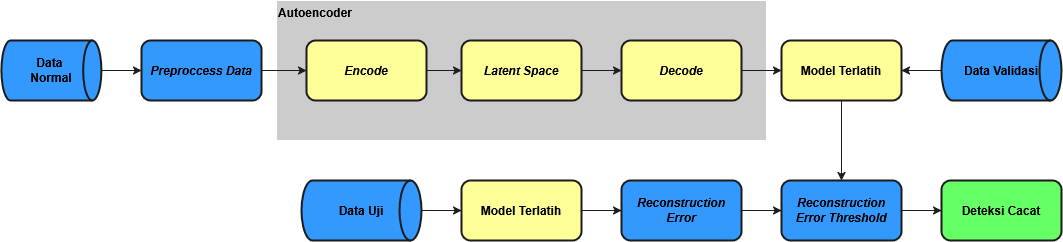
\includegraphics[width=\textwidth]{gambar/pipeline_autoencoder.png}
%   \caption{Diagram \textit{pipeline} pelatihan model deteksi cacat}
%   \label{fig:pipeline-autoencoder}
% \end{figure}
% \vspace{-1em}

\begin{figure}[H]
  \centering
  \begin{tikzpicture}[
      every node/.style={font=\fontsize{9}{11}\selectfont},
      node distance = 1cm and 2cm
    ]
    \node (data-normal) [data] {Data Normal};
    \node (preprocess) [pipeline-box, fill=cyan!50, below=of
    data-normal] {\textit{Preprocess Data}};
    \node (encode) [pipeline-box, fill=yellow!50, below=of
    preprocess] {\textit{Encode}};
    \node (latent-space) [pipeline-box, fill=yellow!50, below=of
    encode] {Ruang Laten};
    \node (decode) [pipeline-box, fill=yellow!50, below=of
    latent-space] {\textit{Decode}};
    \node (model-terlatih) [pipeline-box, fill=yellow!50, below=of
    decode] {Model Terlatih};
    \node (data-validasi) [data, below=of
    model-terlatih] {Data Validasi};

    \node (data-uji) [data, left=of encode] {Data Uji};
    \node (model-terlatih2) [pipeline-box, fill=cyan!50, below=of
    data-uji] {Model Terlatih};
    \node (reconstruction) [pipeline-box, align=center, fill=cyan!50, below=of
    model-terlatih2]
    {\textit{Reconstruction} \\ \textit{Error}};
    \node (threshold) [pipeline-box, align=center, fill=cyan!50, below=of
    reconstruction]
    {\textit{Reconstruction Error} \\ \textit{Threshold}};
    \node (deteksi-cacat) [pipeline-box, fill=green!50, below=of
    threshold] {Deteksi Cacat};

    % Arrow
    \draw [arrow] (data-normal) -- (preprocess);
    \draw [arrow] (preprocess) -- (encode);
    \draw [arrow] (preprocess) -- (encode);
    \draw [arrow] (encode) -- (latent-space);
    \draw [arrow] (latent-space) -- (decode);
    \draw [arrow] (decode) -- (model-terlatih);
    \draw [arrow] (data-validasi) -- (model-terlatih);
    \draw [arrow] (data-uji) -- (model-terlatih2);
    \draw [arrow] (model-terlatih2) -- (reconstruction);
    \draw [arrow] (reconstruction) -- (threshold);
    \draw [arrow] (model-terlatih) -- (threshold);
    \draw [arrow] (threshold) -- (deteksi-cacat);
  \end{tikzpicture}
  \caption{Diagram alur pelatihan model deteksi cacat}
  \label{fig:pipeline-autoencoder}
\end{figure}
\vspace{-1em}

\vspace{1em}

\subsection{Bagan Alir Sistem Kerja Alat}
Alur kerja sistem dimulai dari pengambilan citra oleh kamera,
pendeteksian kontainer menggunakan YOLO dan klasifikasi kecacatan
oleh \textit{autoencoder}. Berdasarkan hasil tersebut, lengan robot
memindahkan kontainer ke wadah yang sesuai. Data hasil klasifikasi
dikirim ke \textit{web server} untuk ditampilkan secara
\textit{real-time}. Alur kerja sistem secara keseluruhan
ditunjukkan pada Gambar \ref{fig:bagan-alir-kerja}.

% \begin{figure}[H]
%   \centering
%   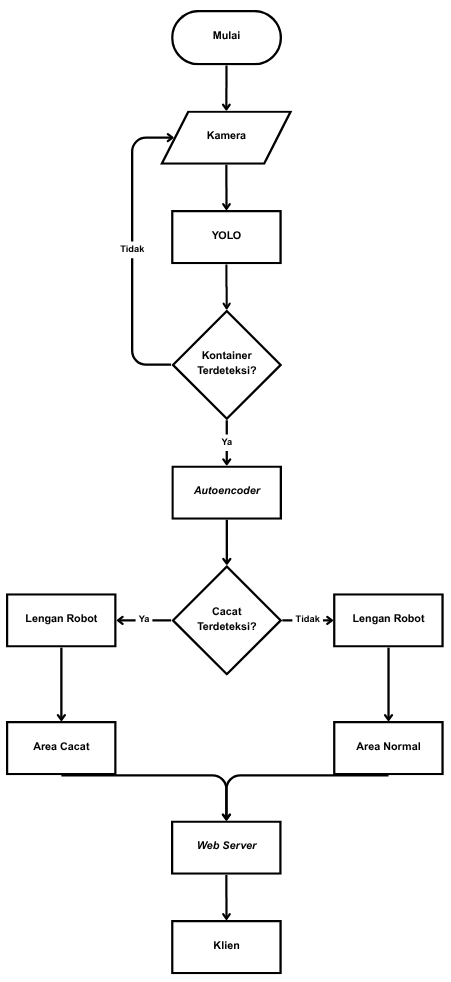
\includegraphics[width=0.7\textwidth]{gambar/flowchart.png}
%   \caption{Bagan alir sistem kerja alat}
%   \label{fig:bagan-alir-kerja}
% \end{figure}
% \vspace{-1em}

\begin{figure}[H]
  \centering

  \begin{tikzpicture}[
      every node/.style={font=\fontsize{9}{11}\selectfont},
      node distance = 0.75cm and 1.5cm
    ]
    \node (mulai) [startstop] {Mulai};
    \node (kamera) [input, below=of mulai] {Kamera};
    \node (yolo) [process, below=of kamera] {YOLO};
    \node (kontainer-terdeteksi) [decision, align=center, below=of yolo]
    {Kontainer \\ Terdeteksi?};
    \node (autoencoder) [process, below=of kontainer-terdeteksi]
    {\textit{Autoencoder}};

    \node (cacat-terdeteksi) [decision, align=center, below=of autoencoder]
    {Cacat \\ Terdeteksi?};
    \node (lengan-cacat) [process, left=of cacat-terdeteksi] {Lengan Robot};
    \node (area-cacat) [process, below=of lengan-cacat] {Area Cacat};
    \node (lengan-normal) [process, right=of cacat-terdeteksi] {Lengan Robot};
    \node (area-normal) [process, below=of lengan-normal] {Area Normal};

    \node (web) [process, below left=of area-normal] {\textit{Web Server}};
    \node (klien) [process, below=of web] {Klien};
    \node (selesai) [startstop, below=of klien] {Selesai};

    % Arrow
    \draw [arrow] (mulai) -- (kamera);
    \draw [arrow] (kamera) -- (yolo);
    \draw [arrow] (yolo) -- (kontainer-terdeteksi);

    \draw [arrow] (kontainer-terdeteksi) -- node[midway,
    xshift=0.3cm]{Iya} (autoencoder);
    \draw [arrow] (kontainer-terdeteksi.west) -- node[midway,
    yshift=0.25cm]{Tidak}
    ($(kontainer-terdeteksi.west)+(-2cm,0)$) |- (kamera.west);

    \draw [arrow] (autoencoder) -- (cacat-terdeteksi);
    \draw [arrow] (cacat-terdeteksi.east) -- node[midway, yshift=0.25cm]{Tidak}
    (lengan-normal);
    \draw [arrow] (cacat-terdeteksi.west) -- node[midway,
    yshift=0.25cm]{Iya} (lengan-cacat);
    \draw [arrow] (lengan-cacat) -- (area-cacat);
    \draw [arrow] (lengan-normal) -- (area-normal);

    \draw [arrow] (area-cacat.south) --
    ($(area-cacat.south)+(0,-0.4)$) -| (web.north);
    \draw [arrow] (area-normal.south) --
    ($(area-normal.south)+(0,-0.4)$) -| (web.north);

    \draw [arrow] (web) -- (klien);
    \draw [arrow] (klien) -- (selesai);

  \end{tikzpicture}
  \caption{Bagan alir sistem kerja alat}
  \label{fig:bagan-alir-kerja}
\end{figure}
\vspace{-1em}
